\documentclass[]{article}
\usepackage{lmodern}
\usepackage{amssymb,amsmath}
\usepackage{ifxetex,ifluatex}
\usepackage{fixltx2e} % provides \textsubscript
\ifnum 0\ifxetex 1\fi\ifluatex 1\fi=0 % if pdftex
  \usepackage[T1]{fontenc}
  \usepackage[utf8]{inputenc}
\else % if luatex or xelatex
  \ifxetex
    \usepackage{mathspec}
  \else
    \usepackage{fontspec}
  \fi
  \defaultfontfeatures{Ligatures=TeX,Scale=MatchLowercase}
\fi
% use upquote if available, for straight quotes in verbatim environments
\IfFileExists{upquote.sty}{\usepackage{upquote}}{}
% use microtype if available
\IfFileExists{microtype.sty}{%
\usepackage[]{microtype}
\UseMicrotypeSet[protrusion]{basicmath} % disable protrusion for tt fonts
}{}
\PassOptionsToPackage{hyphens}{url} % url is loaded by hyperref
\usepackage[unicode=true]{hyperref}
\hypersetup{
            pdftitle={Results},
            pdfborder={0 0 0},
            breaklinks=true}
\urlstyle{same}  % don't use monospace font for urls
\usepackage[margin=1in]{geometry}
\usepackage{graphicx,grffile}
\makeatletter
\def\maxwidth{\ifdim\Gin@nat@width>\linewidth\linewidth\else\Gin@nat@width\fi}
\def\maxheight{\ifdim\Gin@nat@height>\textheight\textheight\else\Gin@nat@height\fi}
\makeatother
% Scale images if necessary, so that they will not overflow the page
% margins by default, and it is still possible to overwrite the defaults
% using explicit options in \includegraphics[width, height, ...]{}
\setkeys{Gin}{width=\maxwidth,height=\maxheight,keepaspectratio}
\IfFileExists{parskip.sty}{%
\usepackage{parskip}
}{% else
\setlength{\parindent}{0pt}
\setlength{\parskip}{6pt plus 2pt minus 1pt}
}
\setlength{\emergencystretch}{3em}  % prevent overfull lines
\providecommand{\tightlist}{%
  \setlength{\itemsep}{0pt}\setlength{\parskip}{0pt}}
\setcounter{secnumdepth}{0}
% Redefines (sub)paragraphs to behave more like sections
\ifx\paragraph\undefined\else
\let\oldparagraph\paragraph
\renewcommand{\paragraph}[1]{\oldparagraph{#1}\mbox{}}
\fi
\ifx\subparagraph\undefined\else
\let\oldsubparagraph\subparagraph
\renewcommand{\subparagraph}[1]{\oldsubparagraph{#1}\mbox{}}
\fi

% set default figure placement to htbp
\makeatletter
\def\fps@figure{htbp}
\makeatother

\usepackage{booktabs}
\usepackage{longtable}
\usepackage{array}
\usepackage{multirow}
\usepackage{wrapfig}
\usepackage{float}
\usepackage{colortbl}
\usepackage{pdflscape}
\usepackage{tabu}
\usepackage{threeparttable}
\usepackage{threeparttablex}
\usepackage[normalem]{ulem}
\usepackage{makecell}
\usepackage{xcolor}

\title{Results}
\author{}
\date{\vspace{-2.5em}}

\begin{document}
\maketitle

An introduction to results. A description of each one of the results.

\subsubsection{Participants}\label{participants}

\begin{table}

\caption{\label{tab:unnamed-chunk-1}Participants demographics}
\centering
\begin{tabular}[t]{l|l|l|l|l|l|l|l|l|l}
\hline
participant & gender & age & occupation & country of origin & type accomodation & people in accomodation & inhabitants in accomodation & first session & helpers\\
\hline
\rowcolor{gray!6}  1 & male & 25 & PhD student & Indonesia & house & 2 & professionals & reg & \\
\hline
2 & non binary & 28 & PhD student & Germany & house & 4 & students & new & \\
\hline
\rowcolor{gray!6}  3 & male & 19 & Undergraduate student & Hong Kong & flat & 6 & students & reg & \\
\hline
4 & female & 50 & Impact officer & USA & house & 4 & family & new & \\
\hline
\rowcolor{gray!6}  5 & male & 30 & Administrator & UK & house & 2 & couple & reg & new\\
\hline
6 & female & 32 & Jobseeker & Hong Kong & house & 4 & professionals & reg & \\
\hline
\rowcolor{gray!6}  7 & male & 32 & PhD student & Iraq & flat & 3 & family & reg & \\
\hline
8 & female & 33 & PhD student & Russia & flat & 1 & individual & reg & \\
\hline
\rowcolor{gray!6}  9 & female & 29 & Invigilator & Mexico & flat & 2 & couple & new & reg \& new\\
\hline
10 & male & 29 & PhD student & Greece & flat & 2 & couple & reg & \\
\hline
\rowcolor{gray!6}  11 & female & 29 & PhD student & Bosnia and Herzegovina & flat & 2 & couple & new & \\
\hline
12 & male & 46 & Researcher & Mexico & house & 5 & family & reg & \\
\hline
\rowcolor{gray!6}  13 & female & 29 & Lecturer & UK & house & 2 & couple & new & new\\
\hline
14 & female & 35 & Housewife & Mexico & house & 4 & family & new & \\
\hline
\rowcolor{gray!6}  15 & female & 72 & Retired & Puerto Rico & house & 2 & couple & new & \\
\hline
16 & female & 40 & Housewife & Mexico & house & 3 & family & reg & \\
\hline
\rowcolor{gray!6}  17 & female & 32 & Research fellow & Ireland & house & 6 & professionals & reg & \\
\hline
18 & female & 26 & Food scientist & UK & house & 3 & professionals & new & reg \& new\\
\hline
\rowcolor{gray!6}  19 & female & 37 & Supply chain manager & China & house & 3 & family & new & \\
\hline
20 & female & 46 & School director & UK & house & 3 & family & reg & \\
\hline
\end{tabular}
\end{table}

\subsubsection{Recipes}\label{recipes}

Add recipe source

\begin{table}

\caption{\label{tab:unnamed-chunk-2}List of recipes}
\centering
\begin{tabular}[t]{l|l|l}
\hline
session & regular & new\\
\hline
\rowcolor{gray!6}  1 & chicken coconut curry & mac and cheese\\
\hline
2 & chickpeas curry with rice & butternut squash curry with coconut milk\\
\hline
\rowcolor{gray!6}  3 & pasta bolognesa & stir fry chicken, rice and peas\\
\hline
4 & green vegs soup & creamy tomato and chorizo rigatoni\\
\hline
\rowcolor{gray!6}  5 & pasta bolognesa & mexican chicken stew\\
\hline
6 & noddles with vegetables (spaggetti) & chicken gyros\\
\hline
\rowcolor{gray!6}  7 & oven roasted chicken & pomegranate rice and salad\\
\hline
8 & scrambled eggs with vegs & ricotta pancakes\\
\hline
\rowcolor{gray!6}  9 & chicken fajitas with rice and fried beans & beef, bean, and beer chili\\
\hline
10 & scrambled eggs with vegs and sausages & mushroom risotto\\
\hline
\rowcolor{gray!6}  11 & pasta bolognesa with vegs & crispy five-spice chicken\\
\hline
12 & minced vegs with vegetables tacos & spanish tortilla (potatoes omelette)\\
\hline
\rowcolor{gray!6}  13 & creamy risssoto with vegs and prawns & keralan chicken curry\\
\hline
14 & vegetable-based stew & cream of spinach soup\\
\hline
\rowcolor{gray!6}  15 & rice with chickpeas (puerto rican rice) & spinach and chickpea soup\\
\hline
16 & roasted chicken and roasted vegetables & white beans with artichokes\\
\hline
\rowcolor{gray!6}  17 & shepherd's pie & szechuan cabbage and crispy chilli beef\\
\hline
18 & pasta carbonara \& pasta napolitana & malfatti ricotta and spinach \& hummus\\
\hline
\rowcolor{gray!6}  19 & shepherd's pie & prawn and black beans curry\\
\hline
20 & creamy chicken pasta & spicy beef with coriander relish\\
\hline
\end{tabular}
\end{table}

\subsubsection{Source of recipes}\label{source-of-recipes}

Description of the recipe source

\begin{table}

\caption{\label{tab:unnamed-chunk-3}Source of recipes}
\centering
\begin{tabular}[t]{l|l|l|l|l}
\hline
session & instrument & tool & source & duration\\
\hline
\rowcolor{gray!6}  1 & laptop & website & epicurious.com & 70\\
\hline
2 & phone & website & shefskitchen.com & \\
\hline
\rowcolor{gray!6}  3 & phone & website & studenthut.com & \\
\hline
4 & phone & website & kitchensanctuary.com & 25\\
\hline
\rowcolor{gray!6}  5 & phone & website & bbc.com & 45\\
\hline
6 & book &  & The Mob Kitchen. Ben Lebus & 30\\
\hline
\rowcolor{gray!6}  7 & notebook & handwritten & partner's recipe & \\
\hline
8 & phone & website & allrecipes.com & 25\\
\hline
\rowcolor{gray!6}  9 & laptop & website and video & foodwishes.com and youtube/foodwishes & \\
\hline
10 & tablet & website and video & akispetretzikis.com and youtube/akispetretzikis & 55\\
\hline
\rowcolor{gray!6}  11 & book &  & The 20-minute Cookbook Jenni Fleetwood & 20\\
\hline
12 & laptop & video & youtube/RecetasdeCocina & \\
\hline
\rowcolor{gray!6}  13 & laptop and tablet & website & bbc.com & 120\\
\hline
14 & book &  &  & 55\\
\hline
\rowcolor{gray!6}  15 & book &  & The Food of Spain. A celebration. Claudia Roden & \\
\hline
16 & book &  & River cottage Veg Everyday. Hugh Fearnley-Whittingstall & \\
\hline
\rowcolor{gray!6}  17 & notebook & handwritten & restaurant's recipe & \\
\hline
18 & phone & website & abelandcole.com & 40\\
\hline
\rowcolor{gray!6}  19 & sheet &  & helloFresh & 15\\
\hline
20 & book &  & Bills Open Kitchen. Bill Granger & \\
\hline
\end{tabular}
\end{table}

\subsubsection{Inventory CPGs}\label{inventory-cpgs}

\begin{table}

\caption{\label{tab:unnamed-chunk-4}Inventory CPGs}
\centering
\begin{tabular}[t]{l|l}
\hline
participant & CPGs\\
\hline
\rowcolor{gray!6}  1 & 121\\
\hline
2 & 199\\
\hline
\rowcolor{gray!6}  3 & 38\\
\hline
4 & 158\\
\hline
\rowcolor{gray!6}  5 & 266\\
\hline
6 & 204\\
\hline
\rowcolor{gray!6}  7 & 155\\
\hline
8 & 220\\
\hline
\rowcolor{gray!6}  9 & 196\\
\hline
10 & 138\\
\hline
\rowcolor{gray!6}  11 & 208\\
\hline
12 & 206\\
\hline
\rowcolor{gray!6}  13 & 179\\
\hline
14 & 301\\
\hline
\rowcolor{gray!6}  15 & 254\\
\hline
16 & 212\\
\hline
\rowcolor{gray!6}  17 & 423\\
\hline
18 & 99\\
\hline
\rowcolor{gray!6}  19 & 189\\
\hline
20 & 272\\
\hline
\end{tabular}
\end{table}

\begin{center}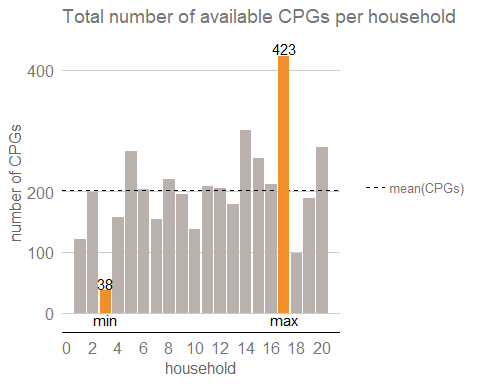
\includegraphics{test_files/figure-latex/unnamed-chunk-5-1} \end{center}

\subsubsection{List of items}\label{list-of-items}

\begin{table}

\caption{\label{tab:unnamed-chunk-6}List of consumer packaged goods}
\centering
\begin{tabular}[t]{>{\bfseries}l|l|>{\bfseries}l|l|>{\bfseries}l|l|l|l|l}
\hline
item & type & sub-cat & item & type & sub-cat & item & type & sub-cat\\
\hline
bread & c & breads & disposables & c & disposables & fiveSpicesSeasoning & c & spice\\
\hline
cake & c & breads & beer & c & drinks & garlicPwd & c & spice\\
\hline
chips & c & breads & cider & c & drinks & ginger & c & spice\\
\hline
tortillas & c & breads & coffee & c & drinks & goyaSeasoning & c & spice\\
\hline
bakingPwd & c & cereals & iceRocks & c & drinks & italianSpices & c & spice\\
\hline
cornFlour & c & cereals & juice & c & drinks & marjoran & c & spice\\
\hline
flour & c & cereals & soda & c & drinks & masalaSpices & c & spice\\
\hline
macarroni & c & cereals & spirit & c & drinks & oregano & c & spice\\
\hline
noodles & c & cereals & tea & c & drinks & paprika & c & spice\\
\hline
nuts & c & cereals & wine & c & drinks & rosemary & c & spice\\
\hline
panko & c & cereals & food & c & food & salt & c & spice\\
\hline
rice & c & cereals & kiwi & c & fruit & seasoning & c & spice\\
\hline
rigatoni & c & cereals & lemon & c & fruit & seasoningChicken & c & spice\\
\hline
spaghetti & c & cereals & lime & c & fruit & spice\_ui & c & spice\\
\hline
cleaningLiquid & c & cleaningProduct & beans & c & legumes & sugar & c & spice\\
\hline
cloth & c & cleaningProduct & chickpeas & c & legumes & turmeric & c & spice\\
\hline
dWashL & c & cleaningProduct & greenBeans & c & legumes & whitePepper & c & spice\\
\hline
gloves & c & cleaningProduct & pen & c & nonCooking & artichoke & c & veg\\
\hline
hWashL & c & cleaningProduct & butter & c & oils\&fats & asparagus & c & veg\\
\hline
kitchenRoll & c & cleaningProduct & lard & c & oils\&fats & aubergine & c & veg\\
\hline
napkins & c & cleaningProduct & lighter & c & oils\&fats & avocado & c & veg\\
\hline
soap & c & cleaningProduct & oil & c & oils\&fats & basil & c & veg\\
\hline
sponge & c & cleaningProduct & oilFlavoured & c & oils\&fats & beanSprouts & c & veg\\
\hline
toiletPaper & c & cleaningProduct & bacon & c & proteins & bellPepper & c & veg\\
\hline
water & c & cleaningProduct & beef & c & proteins & butternutSquash & c & veg\\
\hline
wipes & c & cleaningProduct & chicken & c & proteins & cabbage & c & veg\\
\hline
alioli & c & condiment & chorizo & c & proteins & carrots & c & veg\\
\hline
cilantroBase & c & condiment & eggs & c & proteins & celery & c & veg\\
\hline
coconutCream & c & condiment & ham & c & proteins & chillies & c & veg\\
\hline
fishSauce & c & condiment & mincedMeat & c & proteins & chineseGreens & c & veg\\
\hline
hoisinSauce & c & condiment & nuggets & c & proteins & coriander & c & veg\\
\hline
hotSauce & c & condiment & prawns & c & proteins & corn & c & veg\\
\hline
hummus & c & condiment & sausage & c & proteins & courgette & c & veg\\
\hline
jam & c & condiment & pizza & c & readyToEat & cucumber & c & veg\\
\hline
mappleSyrup & c & condiment & riceQuinoa & c & readyToEat & frozenVegs & c & veg\\
\hline
oysterSauce & c & condiment & basilPwd & c & spice & garlic & c & veg\\
\hline
soySauce & c & condiment & blackPepper & c & spice & greenSnaps & c & veg\\
\hline
tahini & c & condiment & bouillon & c & spice & kale & c & veg\\
\hline
tomatoesProcessed & c & condiment & cardamon & c & spice & leeks & c & veg\\
\hline
tomatoesSauce & c & condiment & caribeanSpices & c & spice & lettuce & c & veg\\
\hline
vinegar & c & condiment & cayenne & c & spice & mint & c & veg\\
\hline
worcestershireSauce & c & condiment & chilliesFlakes & c & spice & mushrooms & c & veg\\
\hline
cheese & c & dairy & chilliesPwd & c & spice & onion & c & veg\\
\hline
cream & c & dairy & chineseSpice & c & spice & potatoes & c & veg\\
\hline
milk & c & dairy & chives & c & spice & spinach & c & veg\\
\hline
yogurt & c & dairy & cinamon & c & spice & springOnion & c & veg\\
\hline
alumFoil & c & disposables & cocoa & c & spice & sweetPotatoes & c & veg\\
\hline
bag & c & disposables & corianderPwd & c & spice & thyme & c & veg\\
\hline
bagFreezer & c & disposables & cumin & c & spice & tomatoes & c & veg\\
\hline
bakingPaper & c & disposables & curry & c & spice & turnip & c & veg\\
\hline
clingFilm & c & disposables & fennel & c & spice &  &  & \\
\hline
\multicolumn{9}{l}{\textsuperscript{*} sub-cat = sub-category}\\
\end{tabular}
\end{table}

\begin{table}

\caption{\label{tab:unnamed-chunk-6}List of utensils}
\centering
\begin{tabular}[t]{>{\bfseries}l|l|>{\bfseries}l|l|>{\bfseries}l|l|l|l|l}
\hline
item & type & sub-cat & item & type & sub-cat & item & type & sub-cat\\
\hline
brush & u & clean & tray & u & heat & eyeGlasses & u & nonCooking\\
\hline
dishTray & u & clean & wok & u & heat & key & u & nonCooking\\
\hline
dustBrush & u & clean & rBook & u & informationAccess & remoteControl & u & nonCooking\\
\hline
dustPan & u & clean & rSheet & u & informationAccess & vaper & u & nonCooking\\
\hline
mop & u & clean & chopSticks & u & manipulate & vessel & u & nonCooking\\
\hline
towel & u & clean & colander & u & manipulate & wallet & u & nonCooking\\
\hline
vacuum & u & clean & cookingSpoon & u & manipulate & canOpener & u & open\\
\hline
bottle & u & contain & cutlery & u & manipulate & scissors & u & open\\
\hline
bowl & u & contain & fork & u & manipulate & blender & u & prepare\\
\hline
boxCondiments & u & contain & holder & u & manipulate & chopB & u & prepare\\
\hline
bucket & u & contain & ladle & u & manipulate & crusher & u & prepare\\
\hline
cup & u & contain & ovenGloves & u & manipulate & grater & u & prepare\\
\hline
glass & u & contain & pastaServer & u & manipulate & jarBlender & u & prepare\\
\hline
glassWine & u & contain & sinkDrainer & u & manipulate & knife & u & prepare\\
\hline
jar & u & contain & spoon & u & manipulate & mortar & u & prepare\\
\hline
jarLid & u & contain & strainer & u & manipulate & peeler & u & prepare\\
\hline
lid & u & contain & tongs & u & manipulate & processor & u & prepare\\
\hline
plate & u & contain & measuringJar & u & measure & smasher & u & prepare\\
\hline
trashB & u & dispose & measuringSpoon & u & measure & apron & u & protect\\
\hline
coffeeMachine & u & heat & scale & u & measure & container & u & store\\
\hline
kettle & u & heat & timer & u & measure & lunchBag & u & store\\
\hline
microwave & u & heat & wristWatch & u & measure & sealingClips & u & store\\
\hline
ovenDish & u & heat & mixingBowl & u & contain & computer & u & tech\\
\hline
pan & u & heat & whisk & u & manipulate & phone & u & tech\\
\hline
pot & u & heat & case & u & nonCooking & radio & u & tech\\
\hline
riceCooker & u & heat & charger & u & nonCooking & smartAssistant & u & tech\\
\hline
teaPot & u & heat & clothes & u & nonCooking & smartWatch & u & tech\\
\hline
toaster & u & heat & documents & u & nonCooking & speaker & u & tech\\
\hline
\multicolumn{9}{l}{\textsuperscript{*} sub-cat = sub-category}\\
\end{tabular}
\end{table}

\begin{table}

\caption{\label{tab:unnamed-chunk-6}List of environment}
\centering
\begin{tabular}[t]{>{\bfseries}l|l|>{\bfseries}l|l|>{\bfseries}l|l|l|l|l}
\hline
item & type & sub-cat & item & type & sub-cat & item & type & sub-cat\\
\hline
cpB & e & store & freezer & e & store & stove & e & heat\\
\hline
dw & e & store & fridge & e & store & washingMachine & e & nonCooking\\
\hline
extractorFan & e & support & lightSwitch & e & nonCooking & window & e & nonCooking\\
\hline
faucet & e & clean & oven & e & heat & dishWasher & e & clean\\
\hline
fireAlarm & e & nonCooking & plan & e & nonCooking &  &  & \\
\hline
\multicolumn{9}{l}{\textsuperscript{*} sub-cat = sub-category}\\
\end{tabular}
\end{table}

\subsubsection{Items by type}\label{items-by-type}

Table. Types of CPGs

item

count

percent

breads

4

{2.6}

cereals

10

{6.6}

cleaningProduct

12

{7.9}

condiment

16

{10.5}

dairy

4

{2.6}

disposables

6

{3.9}

drinks

9

{5.9}

food

1

{0.7}

fruit

3

{2.0}

legumes

3

{2.0}

nonCooking

1

{0.7}

oils\&fats

5

{3.3}

proteins

10

{6.6}

readyToEat

2

{1.3}

spice

33

{21.7}

veg

33

{21.7}

Table. Types of utensils

item

count

percent

clean

7

{8.2}

contain

12

{14.1}

dispose

1

{1.2}

heat

11

{12.9}

informationAccess

2

{2.4}

manipulate

14

{16.5}

measure

5

{5.9}

nonCooking

10

{11.8}

open

2

{2.4}

prepare

10

{11.8}

protect

1

{1.2}

store

3

{3.5}

tech

7

{8.2}

Table. Types of environment

item

count

percent

clean

2

{14.3}

heat

2

{14.3}

nonCooking

5

{35.7}

store

4

{28.6}

support

1

{7.1}

\subsubsection{Duration recipes}\label{duration-recipes}

\begin{table}

\caption{\label{tab:unnamed-chunk-8}Duration of recipes}
\centering
\begin{tabular}[t]{l|l|l}
\hline
session & regular & new\\
\hline
\rowcolor{gray!6}  1 & 36 & 61\\
\hline
2 & 76 & 81\\
\hline
\rowcolor{gray!6}  3 & 21 & 40\\
\hline
4 & 45 & 52\\
\hline
\rowcolor{gray!6}  5 & 41 & 90\\
\hline
6 & 45 & 90\\
\hline
\rowcolor{gray!6}  7 & 88 & 29\\
\hline
8 & 28 & 34\\
\hline
\rowcolor{gray!6}  9 & 68 & 78\\
\hline
10 & 39 & 111\\
\hline
\rowcolor{gray!6}  11 & 56 & 87\\
\hline
12 & 80 & 126\\
\hline
\rowcolor{gray!6}  13 & 42 & 53\\
\hline
14 & 73 & 58\\
\hline
\rowcolor{gray!6}  15 & 50 & 46\\
\hline
16 & 70 & 47\\
\hline
\rowcolor{gray!6}  17 & 113 & 90\\
\hline
18 & 44 & 80\\
\hline
\rowcolor{gray!6}  19 & 70 & 61\\
\hline
20 & 68 & 17\\
\hline
\end{tabular}
\end{table}

\begin{center}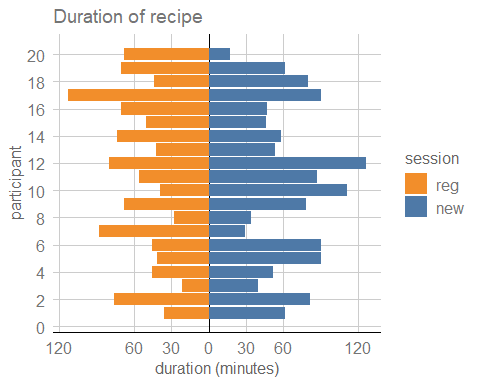
\includegraphics{test_files/figure-latex/unnamed-chunk-9-1} \end{center}

\begin{center}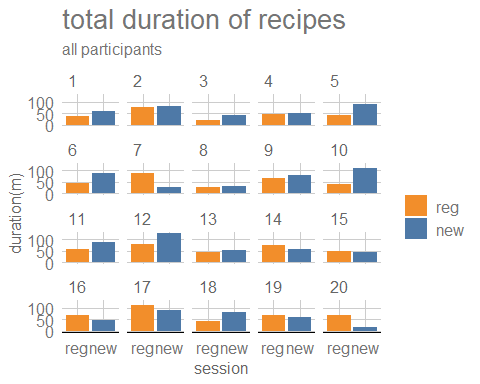
\includegraphics{test_files/figure-latex/unnamed-chunk-10-1} \end{center}

\subsubsection{Items used}\label{items-used}

The list of the items used

\begin{table}

\caption{\label{tab:unnamed-chunk-11}Total number of different items used}
\centering
\begin{tabular}[t]{c|c|c|c|c}
\hline
session & c & u & e & total\\
\hline
all & 970 & 1308 & 496 & 2774\\
\hline
regular & 465 & 567 & 237 & 1269\\
\hline
new & 505 & 741 & 259 & 1505\\
\hline
\multicolumn{5}{l}{\textsuperscript{*} c = CPGs, u = utensil, e = environment}\\
\end{tabular}
\end{table}

\subsubsection{Total number of different items
used}\label{total-number-of-different-items-used}

The total number of different items used were as follows:

\begin{table}

\caption{\label{tab:unnamed-chunk-12}Total number of different items used}
\centering
\begin{tabular}[t]{c|c|c|c|c}
\hline
session & c & u & e & total\\
\hline
all & 970 & 1308 & 496 & 2774\\
\hline
regular & 465 & 567 & 237 & 1269\\
\hline
new & 505 & 741 & 259 & 1505\\
\hline
\multicolumn{5}{l}{\textsuperscript{*} c = CPGs, u = utensil, e = environment}\\
\end{tabular}
\end{table}

\end{document}
